\documentclass[12pt]{article}


% Language setting
% Replace `english' with e.g. `spanish' to change the document language
\usepackage[english]{babel}

% Set page size and margins
% Replace `letterpaper' with `a4paper' for UK/EU standard size
\usepackage[letterpaper,top=2cm,bottom=2cm,left=2cm,right=2cm,marginparwidth=2cm]{geometry}

\usepackage{listings}

% Useful packages
\usepackage{amsmath}
\usepackage{graphicx}
\usepackage[colorlinks=true, allcolors=blue]{hyperref}

\title{Polytechnique Montreal \\
LOG8415E: Lab 2\\
Mapreduce with Hadoop on AWS}

\author{Line Ghanem - 1728134\\Zineddine Aliche - 1949905\\
Mohammed Ramzi Bouthiba - 2065386\\Axelle Pagnier - 2164162}

\begin{document}
\maketitle

\begin{abstract}

\end{abstract}

\section{Setting Up the Environment}


\section{Experiments with WordCount}
\subsection{Hadoop vs. Linux}

 
\subsection{Hadoop vs. Linux}
\section{Hadoop vs. Spark}


\section{Social network friendship recommendation}


\paragraph{}
In this section we will describe a solution to the following problem:
give 10 friends recommendation to each user based on their mutual friends.
For each user we will return the 10 recommendations with home the user has the biggest number of mutual friends. Since we are using Hadoop MapReduce to solve the problem we have divided our implementation in two phases Map and Reduce using the java \textbf{org.apache.hadoop} packages.

The Map section will first map each friend to his first degree friends as follows: \textbf{(UserKey, (Friend, -1))}.
Then, for each friend in the friend list of the user we will create a second degree relationship as follows: \textbf{(Friend1, (Friend2, 1))} and \textbf{(Friend2, (Friend1, 1))}. Note a relationship with 1 means they are second degree friends and a relationship with -1 means they are first degree friends. Note a relationship with 1 means they are second degree friends and a relationship with -1 means they are first degree friends. Each of the entries create in the map phase are added to the context (Figure \ref{fig:map}).

\begin{figure}[h]
  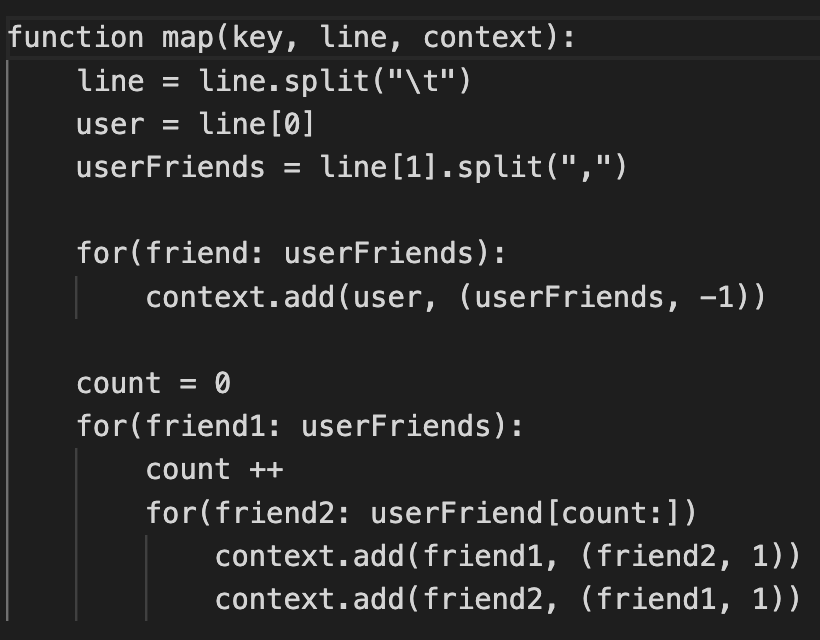
\includegraphics[scale=0.65]{img/map.png}
  \caption{Pseudo code of the mapper function.}
  \label{fig:map}
\end{figure}

In the reduce phase, for each UserKey, we count the number of mutual friends that each user has with the same second degree friend. To do this we will use the context entries created in the map phase. For example, given user A and B if the relationship (A, (D, 1)) is counted 2 times the number of mutual friends between A and D is 2. However, if the following entry existed: (A, (B,-1)); A and B are first degree friends and the count is set to -1 since first degree friends will not be recommended to each other (Figure \ref{fig:reduce}).

\begin{figure}[h]
  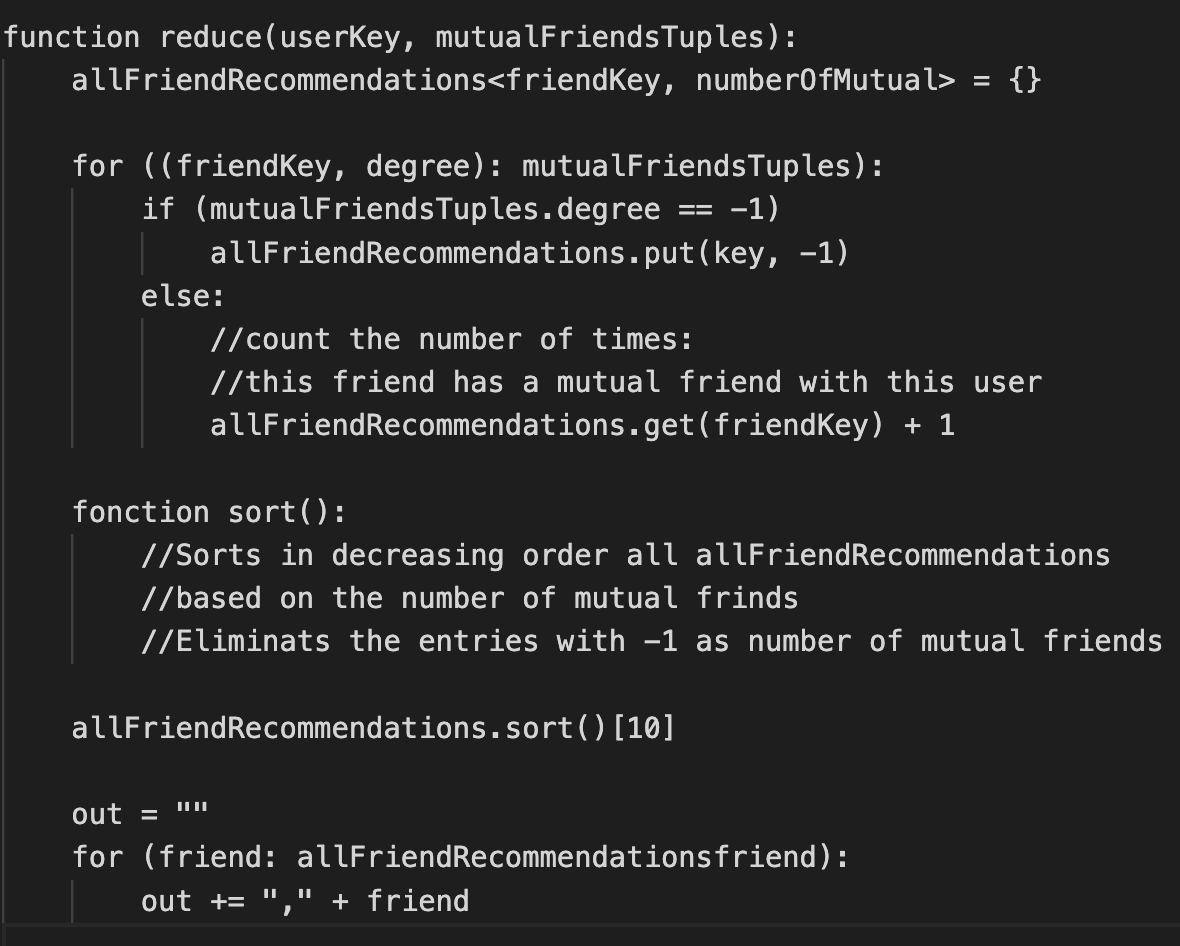
\includegraphics[scale=0.65]{img/reduce.png}
  \caption{Pseudo code of the reducer function.}
  \label{fig:reduce}
\end{figure}

A short example of the logic is seen in Figure \ref{fig:mapreduce}.

\begin{figure}[h]
  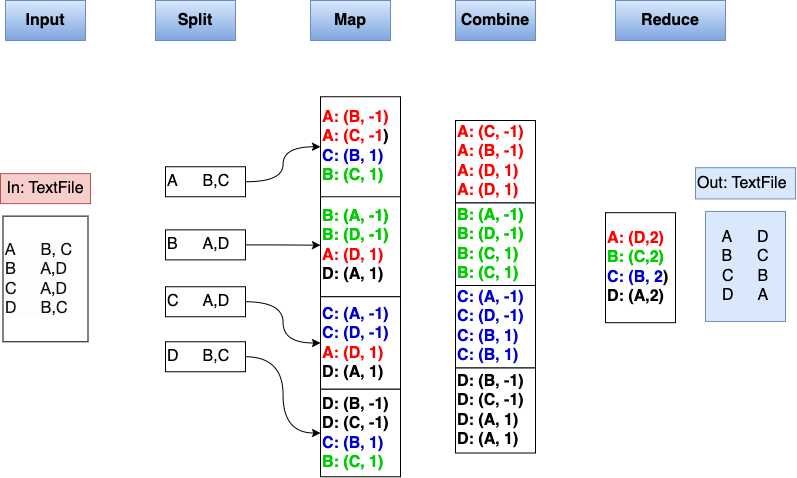
\includegraphics[width=\linewidth]{img/mapreduce.png}
  \caption{Simplified example of the MapReduce solution for the networking problem.}
  \label{fig:mapreduce}
\end{figure}

\paragraph{Results of networking problem:} (Table below)

\begin{center}
\begin{tabular}{ c |c}
  User & Top 10 recommended friends\\
  \hline\hline
  924  &   439,2409,6995,11860,15416,43748,45881\\
  8941  &  8943,8944,8940\\
  8942   & 8939,8940,8943,8944\\
  9019  &  9022,317,9023\\
  9020   & 9021,9016,9017,9022,317,9023\\
  9021   & 9020,9016,9017,9022,317,9023\\
  9022   & 9019,9020,9021,317,9016,9017,9023\\
  9990   & 13134,13478,13877,34299,34485,34642,37941\\
  9992  &  9987,9989,35667,9991\\
  9993  &  9991,13134,13478,13877,34299,34485,34642,37941\\  
\end{tabular}
\end{center}
\section{Conclusion}

\section{Conclusion}



\begin{thebibliography}{9}
 
\end{thebibliography}

\end{document}